\documentclass[10pt]{article}
\usepackage[letterpaper,margin=1in]{geometry}
\usepackage{graphicx}
\newcommand{\figref}[1]{Figure~\ref{fig:#1}}
\title{Implementation of Tokutek Hot Backup}
\author{Bradley C. Kuszmaul}

\input{master-ipe.tex}
\begin{document}
\maketitle

The Tokutek Hot Backup System can back up the file-resident data of an
application, such as MySQL, that runs as a single process.
Applications such as PostgreSQL that operate as multiple processes
could be backed up using a similar scheme with some adaptation.  The
application makes calls to operating system functions such as
\texttt{open()}, \texttt{close()}, \texttt{dup()}, \texttt{unlink()},
\texttt{link()}, \texttt{rename()}, \texttt{read()}, \texttt{write()},
and \texttt{pwrite()}.  The backup system makes a copy of the data of
the application, and as it makes the copy, the backup system
interposes itself in the system functions so that it observes those
calls, and updates the backup copy accordingly.

For example, if there were a 100GB file that the backup system was
backing up, it might take something like 15~minutes to copy the file
to the backup.  If while that copy operates, the application writes
into the file, then the backup system observes the write and arranges
for the newly written data to appear in the backup copy.

The backup system maintains a representation of the underlying file
system, by keeping track of, for example,
\begin{itemize}
\item which open file descriptors (integers) refer to which file description,
\item the read/write offset for each file description,
\item which file name refer to which file in the directory, and
\item which blocks in which files are being written.
\end{itemize}

An example of the state of the hotbackup system is shown in
\figref{overview}, which shows a mapping \citefmap, called fmap,
mapping from file descriptors to DESCRIPTIONs.  In \figref{overview},
file descriptor number~3 points to a DESCRIPTION.

A DESCRIPTION \citedescr comprises an offset \citeoffset, which in
this case is 7. The offset indicates where the next read or write will
occur in the file.  A DESCRIPTION further comprises a pointer
\citesfileptr to an sfile \citesfile.  A DESCRIPTION further contains
a reference count (refcount) \citedrefcount (which equals 1 in this case)
indicating that there is one reference to the description in the fmap.

An SFILE \citesfile comprises rangelocks \citeranges, a set of ranges
that are currently locked.  In this case there are two ranges.  The
first range covers bytes 3--5.  (In our notation, all ranges include
the first value and don't include the last value.  So range 3--5
includes bytes 3 and 4, but not byte 5, for example.)  The second
range covers bytes 18--21.

An SFILE further comprises a set \citefilenames of file names (one
name is shown in this example); a reference count \citesrefcount which
indicates how many descriptions refer to the sfile (one in this case);
and a file identifier (fileid) \citefileid, which comprises a device
number \citedevnum (13 in this case) and inode number \citeinodenum
(1431 in this case).

The system further comprises a directory \citedirectory which maps
from names to SFILES, and an mapping structure called the imap \citeimap that
maps from fileids to SFILES.  The directory provides a way to find an
sfile given a name, and the imap provides a way to find an sfile given
a file identifier.

\begin{figure}
\begin{center}
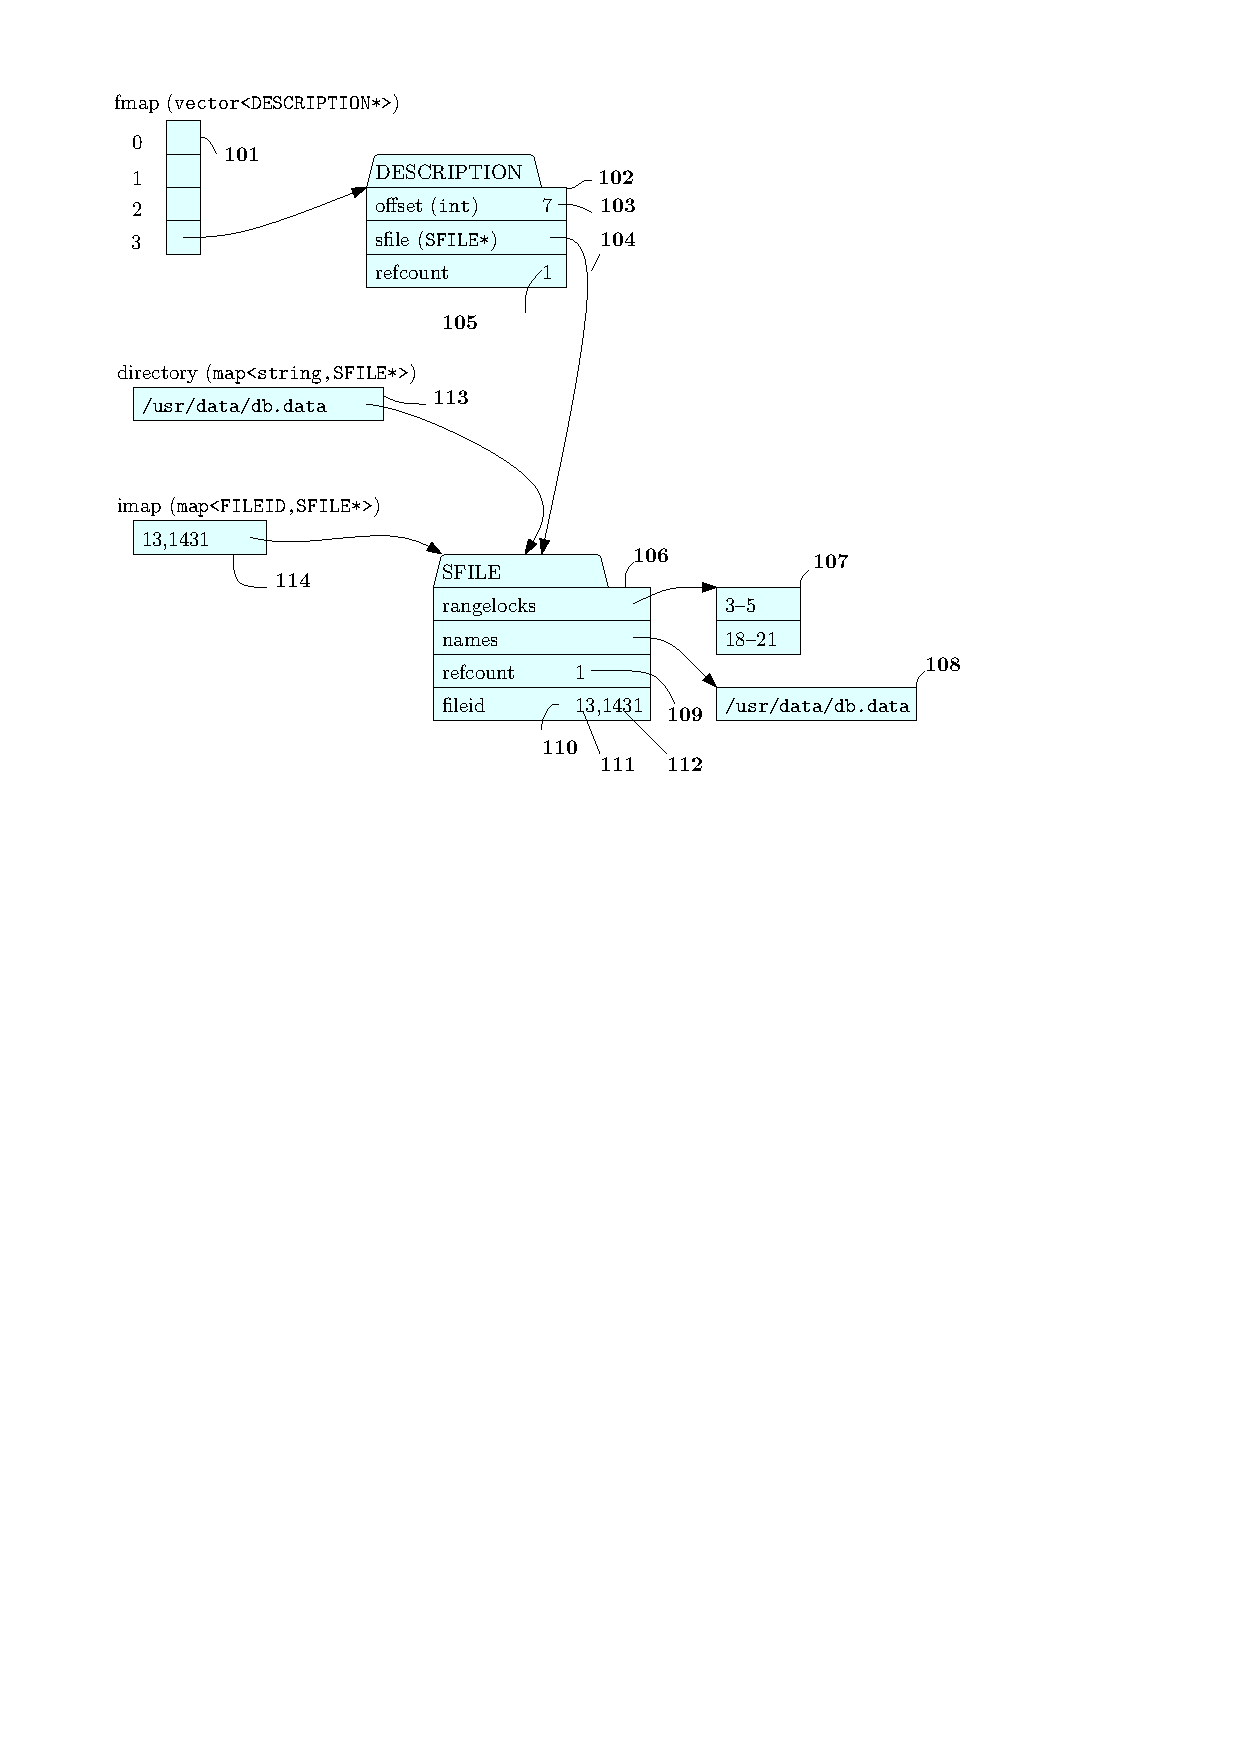
\includegraphics{figures/overview.pdf}
\end{center}
\caption{A typical state of the hot backup system.}
\label{fig:overview}
\end{figure}

In general the hotbackup system is employs the following structures.
\begin{itemize}
\item A file identifier, or \textit{FILEID}, comprises a pair of
  numbers, a device identifier and an inode number.  On many Unix file
  systems, this pair of numbers uniquely identifies a file.  On Unix,
  the device identifer and inode number of a file can be obtained
  using the \texttt{fstat()} system call.  Other file systems, such as
  windows, provide different kinds of FILEIDs, which the system can
  use to identify a file.  In many unix systems, the device number
  might change when the machine restarts.
\item A \textit{file descriptor} is an nonnegative integer that the
  application receives when it calls the \texttt{open()} library
  function.  Typically these integers are relatively small, since in
  many operating systems, the integer that's returned is the smallest
  unused file descriptor.
\item An \textit{fmap} maps the file descriptor to a DESCRIPTION.  The
  system employs a growable vector of pointers to DESCRIPTIONs to implement the fmap.
\item A \textit{DESCRIPTION} comprises
 \begin{itemize}
  \item an offset indicating where the next read or write operation will take place in the file,
  \item a pointer to an SFILE, and
  \item a refcount integer that keeps track of how many fmap entries refer to the description.
 \end{itemize}
\item A \textit{directory} maps file name strings to SFILEs.  The
  directory is an unordered map implmented by a hash table.
\item An \textit{imap} maps FILEIDs to SFILEs.  The imap is an unordered map implemented by a hash table.
\item An \textit{sfile} comprises the following:
 \begin{itemize}
   \item Rangelocks, a set of ranges that are locked.  A range is a
     pair of offsets, $(l,h)$, in a file.  The locked range includes
     byte number $l$ inclusive through byte number $h$ exclusive.  To
     lock the entire file the system may lock the range $(0, \infty)$,
     where $\infty$ is a value that is considered to be larger than
     any offset in a file.  For example, our system uses
     $\infty=2^{64}-1$ which is the largest value that fits in a
     64-bit unsigned value.  The system keeps the locked ranges in an
     ordered map which facilities determining whether a given range
     intersects any range in the rangelocks.  An alternative would be
     for the system to keep the ranges in an unordered vector, which
     could work well, for example, if there were typically relatively
     few locked ranges at any given time.
   \item Names, a set of strings.  A string appears in the names of an
     sfile if and only if, in the directory, the string maps to the
     sfile.  The Names sets is implemented using a hash table.
   \item Refcount, an integer.  This is a count of the number of DESCRIPTIONs that point at the SFILE\@.
   \item A FILEID called fileid, comprising a device number and inode
     number.  If $s$ is an SFILE then
     $\texttt{imap}[s->\mbox{fileid}]=s$, that is in the imap, the file
     identifier of an sfile maps to the sfile.
 \end{itemize}
\end{itemize}

The system maintains several invariants, including the following.  If
$S$ is a string, $F$ is an sfile, integer $I$ is an open file
descriptor pointing at a regular file, and $D$ is an description then:
\begin{enumerate}
\item  $S$ is in $F.\mbox{names}$ if and only if $\mbox{directory}[S]=F$.
\item  $\mbox{fmap}[I]$ is populated (points to a description) and the
description points to an sfile.
\item The number of descriptions that refer to $F$ equals
  $F.\mbox{refcount}$.  (One way for the refcount of $F$ to become
  greater than one is to open the same file twice.)
\item The number of fmap entries that refer to $D$ equals
  $D.\mbox{refcount}$.  (One way for the refcount of $D$ to become
  greater than 1 is to use the \texttt{dup()} or \texttt{dup2()} unix
  system calls.)
\item $\mbox{imap}[F.\mbox{fileid}] = F$.
\item The directory contains exactly the names of files that are open,
  under the names that they were opened through.  But if those names
  change with, e.g., \texttt{rename()} or \texttt{unlink()} we update
  the directory). Recall that when the directory is updated, so must
  the corresponding names set in the relevant sfile.
\end{enumerate}

The system operates as follows:

The manipulation of $F.\mbox{names}$ and $\mbox{directory}[S]$ is done
atomically, and is affected by \texttt{open()}, \texttt{creat()},
\texttt{rename()}, and \texttt{unlink()}.  The system employs a lock,
called the directory lock, which is held while updating
$F.\mbox{names}[S]$ and $\mbox{directory}[S]$.

The system also employs a lock, called the fmap lock, to protect the
fmap from concurrent operations.

The system also employs a lock, called the imap lock, to protect the imap from concurrent operations.

During backup of a file, we go ahead and create a description just as
if the user had opened() the file.  Thus, the refcount of an sfile
will be incremented while the underlying file is being copied during
backup.


\subsection*{Not Doing Backup}

\typeout{Need a picture of an application with backup and describe interposition}.

When we are not doing a backup the system interposes the system calls
performed by the application and operates as follows:

When the user opens a file with $\texttt{open}(S,...)$:
 \begin{enumerate}
 \item The system finds the sfile.  After opening the file, the system
   performs a \texttt{fstat()} on the file, yielding a file identifier.

   Then the system looks in the imap to determine if there is an existing sfile with that file identifier.  If yes, then the refcount is incremented, otherwise an sfile is created with refcount equal to 1.

   The system checks to see if $\mbox{directory}[\mbox{realpath}(S)]$ points at the sfile, if it does not, then the directory is updated as well as the names of the sfile.
   The system creates a description, updates the fmap, and returns the file descriptor to the user.

   \end{enumerate}   
\iffalse
We then look
This is done by looking in the
imap for the inode_info from the result of doing stat on the
opened file descriptor
     that will be returned to the user.    If no such source_file
exists, then create it (it will have a refcount of zero to start with)
             b) Make sure that directory[realpath(S)] points at
source_file.  If it doesn't then make it so.  (Be sure to get the
directory lock for this)
             c) Create a description that points at source_file (now
source_file's reference count is incremented.  Must still hold the
directory lock for this)
             d) Put the description in fmap.  (Probably need only the
fmap_lock for this)
\fi

 \hrule

The hot backup library maintains a ghostly mirror of the file system.  We have several things that mirror the unix file system:
\begin{itemize}
\item filenodes: Keeps track of the range locking for a file.  A file needs to be represented by its device and inode.  Represents a unix file or an inode.
\item directories: The mapping of names to filenodes. Represents the directory heirarchy of the file system, but only the part that involves open files.
\item description: Contains a pair $\left<\mbox{offset},\mbox{filenode}\right>$.  Represents a unix file description.
\item descriptors: Contains a pointer to a description.  For every open open file we have a descriptor.  (In principle several descriptors could point to the same description, but that won't happen until we implement \texttt{dup}).
\end{itemize}

What must happen:
\begin{itemize}
\item On \texttt{write(fd)}: 

 If no backup is running, we must still maintain the descriptoin (increment the offset).

 If backup is running, we must do the write in the destination space.
 (It's possible that the destination file hasn't been copied yet, in
 which case we have a choice: We don't have to mirror the write to the
 backup.

 To handle parallelism: we need to lock the range being written (in the filenode) before doing any of the updates.
  We need to lock the description so that we can update the offset and perform the writes.

\end{itemize}

Direct-IO

\iffalse
\begin{itemize}


  close(i)   decrement fmap[i]->description->source_file->refcount
                    [If the count goes to zero, then remove the names
from the directory, and destroy the source_file.  Don't forget to
update the inode_map.  Remember, when fiddling with names we must
obtain the directory lock.]
                decrement fmap[i]->description->refcount [If it goes
to zero, which is always the case without dup(), then destroy the
description)
                set fmap[i]=NULL.

 rename(S):  Get the directory lock.
                     If directory[S] exists then
                       update the directory and the source_file.names
to the new name.
                     If the file exists in the backup directory, rename it
                     release the directory lock.

 unlink(S):   Get the directory lock.
                    If directory[S] exists then
                      update the directory and the source_file.names
to not have S in it any more.
                    If the file exists in the backup directory, unlink it.


prepare_descriptions() should create the source file with all the
relevant names.  For example if there are 3 names in
description->source_file->names, and all 3 names are in the source
directory, then open the file, and create the corresponding other two
names names with link(2).  If there are 0 names in
description->source_file->names then we must do something special.
For now we can simply arrange not to write anything to the backup for
that prepared description.  Something like your "is_deleted" flag, but
it's on the description.

One thing to worry about:  But maybe not needed for v1:  (Need a
ticket for this).  User could do
 1  fd1 = creat(name1)
 2  link(name1, name2)
 3  close(fd1)

 4  fd1 = open(name1)
 5  unlink(name1)
 6  write(fd1)
 7  fd2 = open(name2)
 8  write(fd2)
 9  write(fd1)

So at step 4 when fd1 is opened, we don't know anything about name2
(step 2 may have been done a long long time ago in another process).
  So when we unlink name1, we are not capturing the writes at step 6
or 9.  But we need to capture those writes.

  To make those work, we need to create a file on the same filesystem
with a name that won't conflict with the backups.  Something like
$(DST)/.backup.23 might work.  We may take the position that we don't
backup files with names like $(SRC)/.backup.*

  So when we unlink a file that has an open file descriptor, instead
of unlinking it in our internal data structures and in the destination
directory we rename it to a new backup name.  At the end of the
backup, we go and unlink all the $(DST)/.backup.* files


You may also want to review the man pages for openat() and linkat().
We may be able to use them for something, but I don't see what.

I think that covers all the cases...  What do you think?

\fi
\end{document}
